%
% 3dimagetemplate.tex
%
% (c) 2021 Prof Dr Andreas Müller, OST Ostschweizer Fachhochschule
%
\documentclass[tikz]{standalone}
\usepackage{times}
\usepackage{amsmath}
\usepackage{txfonts}
\usepackage[utf8]{inputenc}
\usepackage{graphics}
\usetikzlibrary{arrows,intersections,math}
\usepackage{ifthen}
\begin{document}

\newboolean{showgrid}
\setboolean{showgrid}{false}
\def\breite{7}
\def\hoehe{3}

\begin{tikzpicture}[>=latex,thick]

% Povray Bild
\begin{scope}[xshift=-4.66cm]
\node at (0,0) {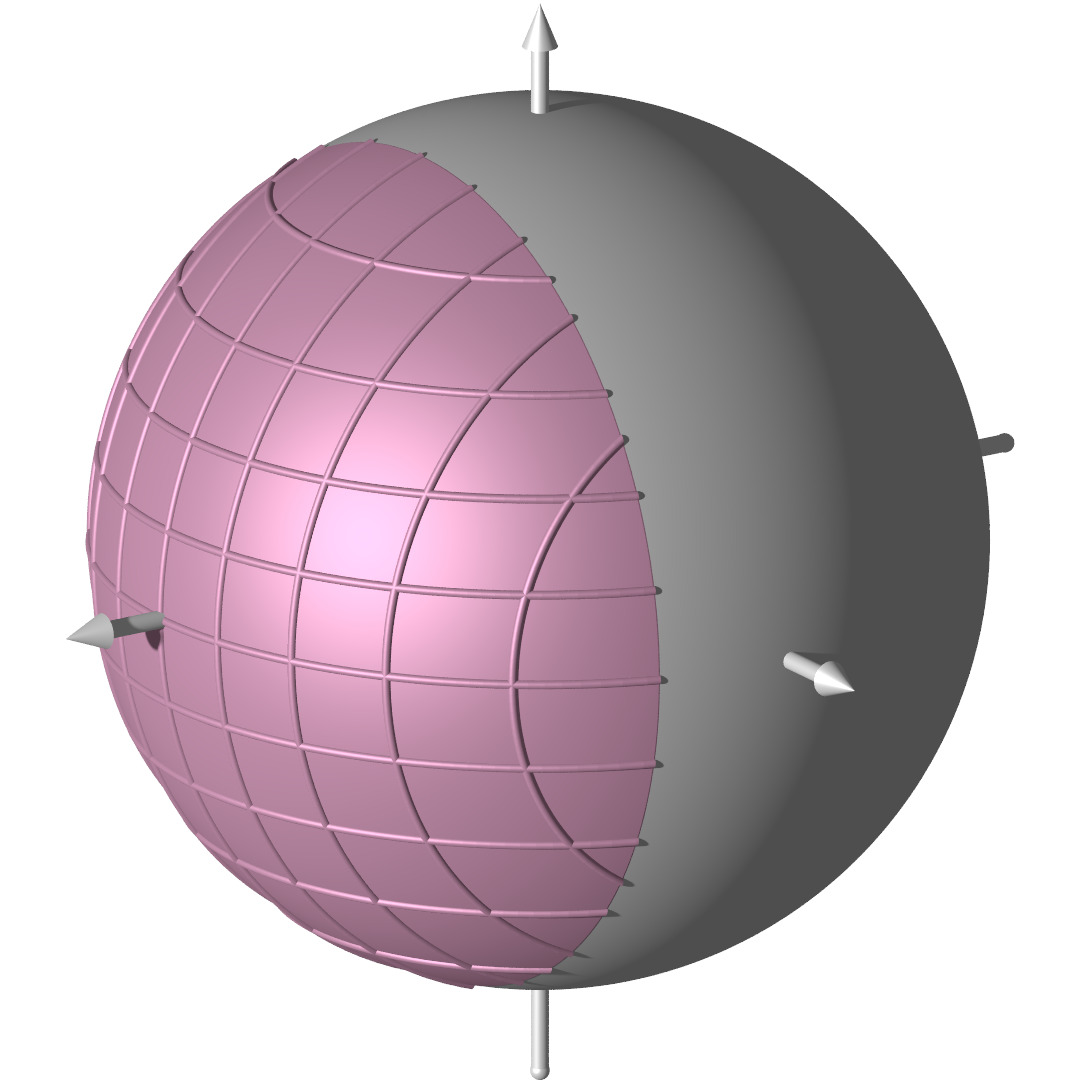
\includegraphics[width=4.66cm]{kugel3.jpg}};
\node at (-2.05,-0.2) {$x$};
\node at (0.2,2.2) {$z$};
\node[color=white] at (1.5,-0.6) {$y$};
\end{scope}

\begin{scope}
\node at (0,0) {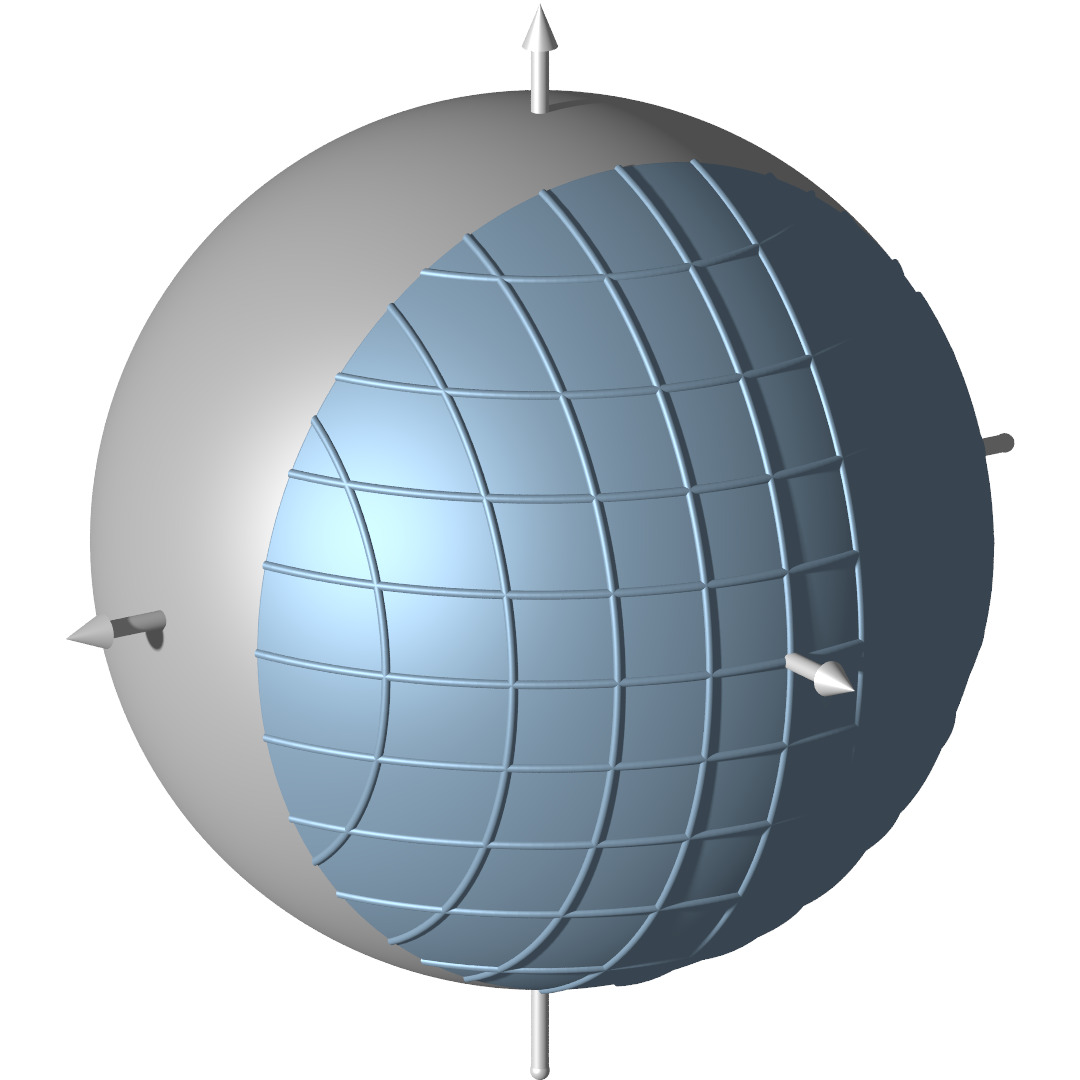
\includegraphics[width=4.66cm]{kugel1.jpg}};
\node at (-2.05,-0.2) {$x$};
\node at (0.2,2.2) {$z$};
\node[color=white] at (1.5,-0.6) {$y$};
\node at (0.7,0.0) {$U_\beta$};
\end{scope}

\begin{scope}[xshift=4.66cm]
\node at (0,0) {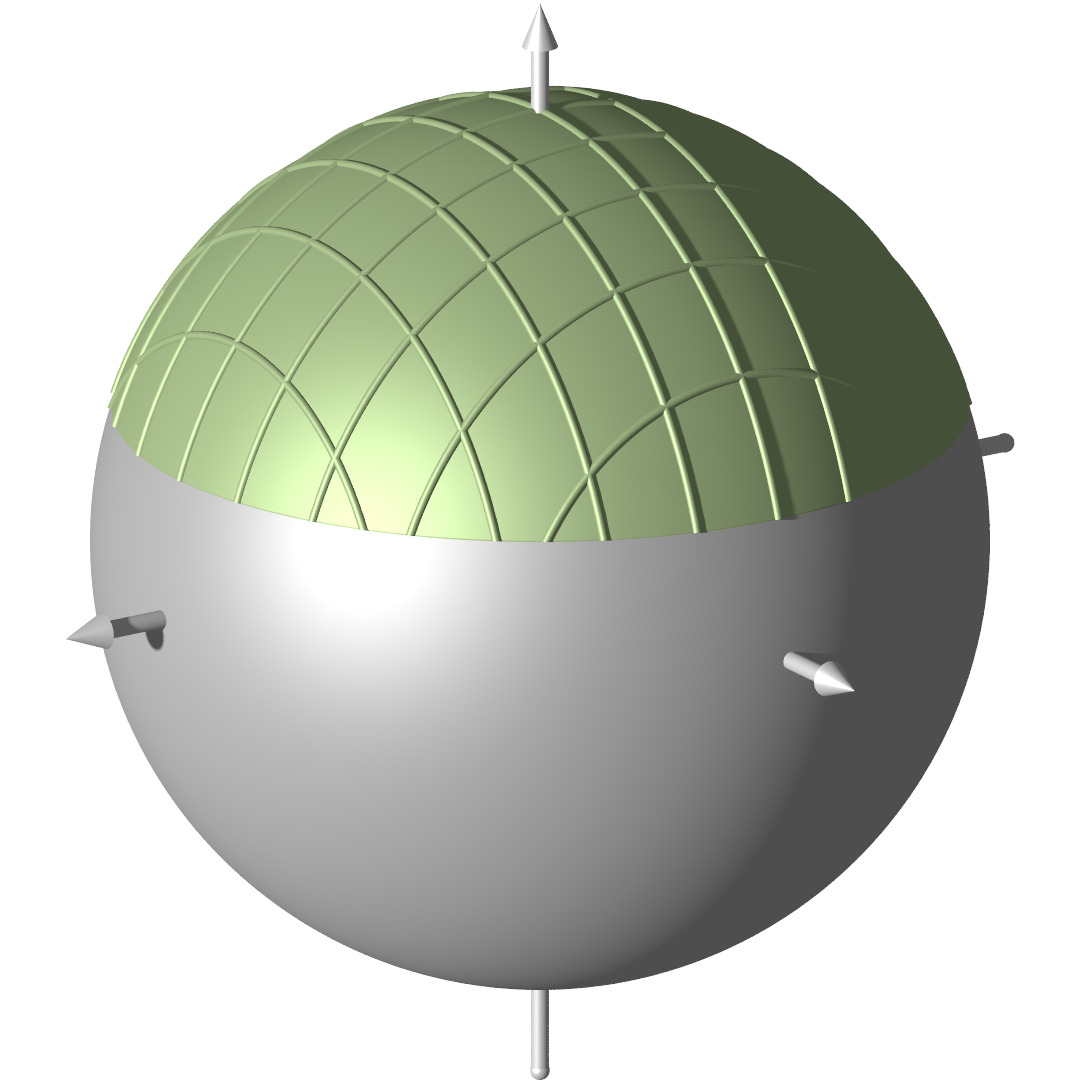
\includegraphics[width=4.66cm]{kugel2.jpg}};
\node at (-2.05,-0.2) {$x$};
\node at (0.2,2.2) {$z$};
\node[color=white] at (1.5,-0.6) {$y$};
\node at (0.1,1.3) {$U_\alpha$};
\end{scope}

% Gitter
\ifthenelse{\boolean{showgrid}}{
\draw[step=0.1,line width=0.1pt] (-\breite,-\hoehe) grid (\breite, \hoehe);
\draw[step=0.5,line width=0.4pt] (-\breite,-\hoehe) grid (\breite, \hoehe);
\draw                            (-\breite,-\hoehe) grid (\breite, \hoehe);
\fill (0,0) circle[radius=0.05];
}{}

\end{tikzpicture}

\end{document}

